\documentclass[a4paper,fleqn]{cas-dc}

%\usepackage[numbers]{natbib}
%\usepackage[authoryear]{natbib}
\usepackage[authoryear,longnamesfirst]{natbib}
\usepackage{titlesec}
\usepackage{graphics}
\usepackage{graphicx}
\usepackage{subfig}

%%%Author definitions
\def\tsc#1{\csdef{#1}{\textsc{\lowercase{#1}}\xspace}}
\tsc{WGM}
\tsc{QE}
\tsc{EP}
\tsc{PMS}
\tsc{BEC}
\tsc{DE}


\begin{document}
\let\WriteBookmarks\relax
\def\floatpagepagefraction{1}
\def\textpagefraction{.001}

% Short title
\shorttitle{\textit{ | Procedia Computer Science 00 (2017) 1–11}}

% Short author
\shortauthors{Yan Huang, Zhipeng Cai and Anu G. Bourgeois.}

% Main title of the paper
\title [mode = title]{Search Locations Safely and Accurately: A Location Privacy Protection
Algorithm with Accurate Service}                      

\tnotetext[1]{Email addresses: chnhuangyan@gmail.com (Yan Huang), zcai@gsu.edu (Zhipeng Cai), abourgeois@cs.gsu.edu (Anu G. Bourgeois)}

\author{Yan Huang}
%  Credit authorship
\credit{Conceptualization of this study, Methodology, Software}

% Second author
\author{Zhipeng Cai}

% Third author
\author{Anu G. Bourgeois}


\credit{Data curation, Writing - Original draft preparation}

% Here goes the abstract
\begin{abstract}
Location-based applications provide convenient services to users. However, they also lead to location privacy leakage. Malicious adversaries may use the leaked information to violate users' privacy in unpredictable ways. Current location protection algorithms use fake or obfuscated locations to query services, thus resulting in inaccurate results. Usually, these algorithms need to sacrifice quality of service to ensure protection. Location searching services (LSSs) is one kind of location-based service (LBS). Users use LSSs to query nearby locations and exact distances to these locations. Thus, any mistake in results can make LSSs useless. Therefore, current location protection algorithms are not suitable for LSSs. In this paper, we propose a novel algorithm to offer protection for LSSs. In the proposed algorithm, users can have accurate LSSs with powerful location privacy protection. Overhead, in terms of data usage, was introduced in this paper to improve the privacy and decrease the Quality Loss (QL) simultaneously. QL can be decreased to zero if users have a good Internet environment. We derive the privacy and QL calculation methods and also use simulations to calculate the expected privacy and QL. The results illustrate that the proposed algorithm has excellent privacy protection and service quality. \\

\begin{center}
    © 2017 Published by Elsevier Ltd.
\end{center}

\end{abstract}


% Keywords
% Each keyword is seperated by \sep
\begin{keywords}
Privacy protection \sep Location search service \sep Location privacy \sep Differential privacy
\end{keywords}

\maketitle
\makeatletter
\renewcommand\section{\@startsection{section}{1}{\z@}%
    {15pt \@plus 3\p@ \@minus 3\p@}%
    {4\p@}%
    {%\let\@hangfrom\relax
     \sectionfont\raggedright\hst[13pt]}}
\renewcommand\subsection{\@startsection{subsection}{2}{\z@}%
    {10pt \@plus 3\p@ \@minus 2\p@}%
    {.1\p@}%
    {%\let\@hangfrom\relax
     \ssectionfont\raggedright }}
\section{Introduction}

With the popularity of smart phones, location-based services (LBSs) can be easily provided to users. Smart phones read lo- cation data from the GPS, then send location data to service providers to query service. Users can get service at anytime and anywhere. For instance, Google Map can lead drivers to their destinations. News apps show what news has happened around users. Weather apps display local weather automatically. Review apps publish crowd-sourced reviews about local businesses such as restaurants,  bars and cafe´s,  and reveal the distance between users and those places. Obviously, those applications make our life more and more convenient. 

However, location information is consistently sent to service providers without protection when users query LBSs, allowing location service providers to collect location information from all users. The collected location information may expose users to customized advertisement, or even be sold to third parties. A worse scenario is location information may be leaked to adversaries with criminal intents. Therefore, many researchers focus on creating location protection algorithms to protect the location privacy of users. Most current research uses fake or obfuscated locations [1, 2, 3], instead of real locations, to query services. Although LBS providers cannot acquire the accurate location information of users protected by location protection mechanisms, query services with obfuscated locations will lead to imprecise service results [4, 5]. There is a trade-off between privacy and service quality. Higher privacy requirements imply greater quality loss [6, 7, 8]. Furthermore, LBSs have many categories such as locating services, navigation services and location searching services. Different kinds of LBSs need different kinds of protection.\\

Location searching services (LSSs) is one kind of location based services (LBSs). Users use LSSs to search nearby location and distances to desired locations. LSSs are widely used in many applications such as Yelp, Hotel.com, Expedia, Groupon and Airbnb. LSSs are also used as functions, such as nearby friends and nearby locations functions of Facebook in mobile applications. For LSSs, users will not tolerate mistakes.example, as shown in Fig. 1 (a), when users use Yelp to find restaurants, they want to know the exact distance to nearby restaurants so that they can pick a close one. If the results are in- accurate, they may pick a remote restaurant. When drivers want to find a gas station on their way (Fig. 1 (b) shows the search results for gas stations), a minor mistake of the search results can lead to an unnecessary detour. As far as we know, existing research does not provide both accurate LSSs and protection in their algorithms.

% Figure with two sub-figures
\begin{figure}
\centering
    \subfloat[Restaurant search in Yelp]
        {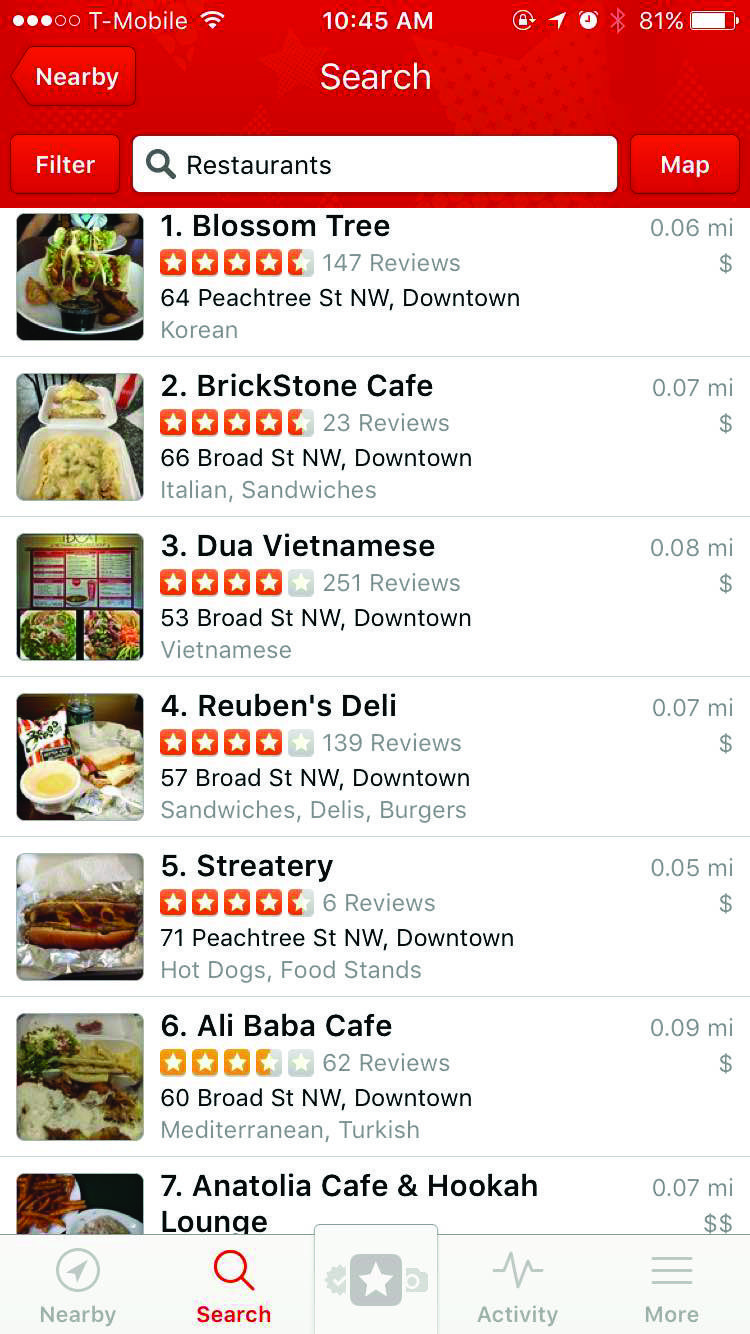
\includegraphics[scale=.9]{figs/fig1-1.png}
            \label{fig:foo-1}
        }
    \hspace{3pt}
    \subfloat[Gas station search in Google]
        {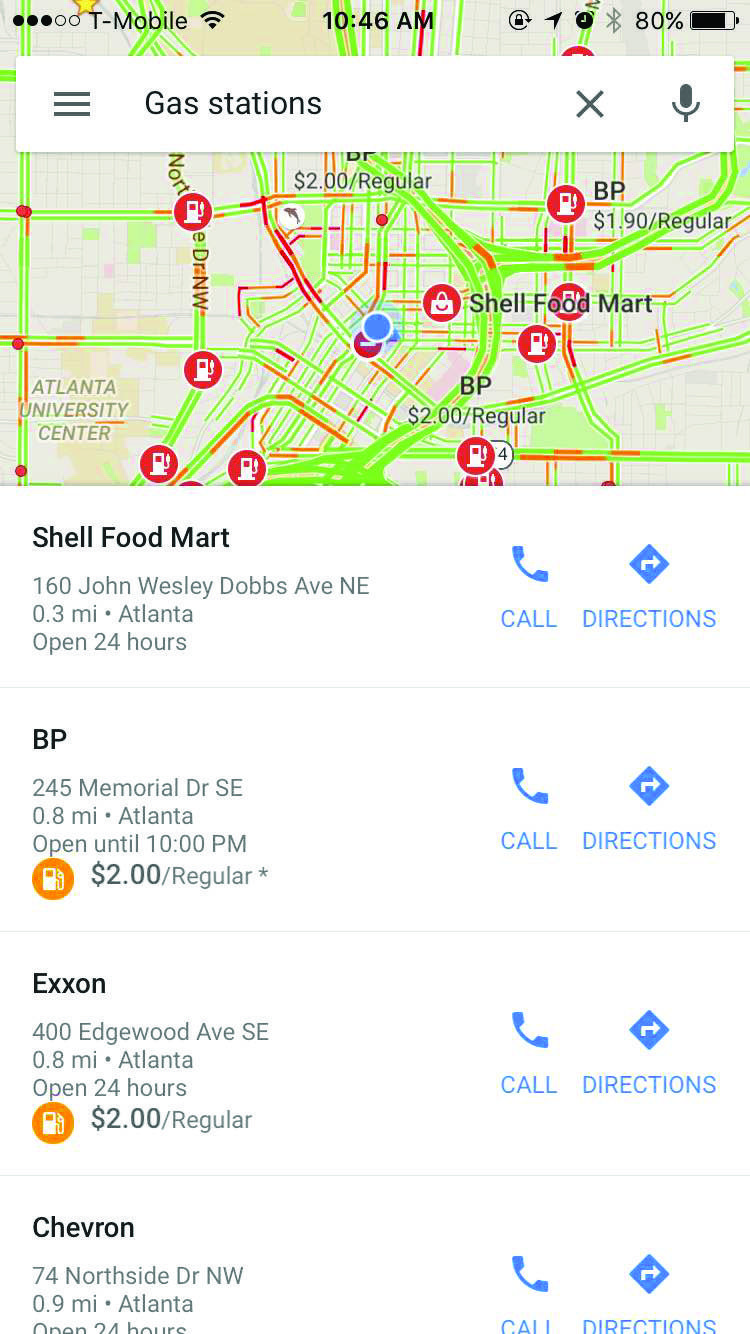
\includegraphics[scale=.9
        ]{figs/fig1-2.png}
            \label{fig:foo-2}
        }
    \caption{ Search results in applications }
    \label{fig:foo}
\end{figure}
In this paper, we introduced an innovative algorithm that provides both accurate LSSs and location privacy protection. Most existing research uses Euclidean distance between real lo- cations and obfuscated locations to define privacy and quality loss. In the proposed algorithm, we introduced new definitions for privacy and quality loss. In addition, the proposed algorithm can provide not only protection for location privacy but also accurate services. Overhead was introduced in this paper to increase the strength of protection and decrease quality loss. Users can get zero quality loss if their Internet connection condition can satisfy the demands of overhead. Even for normal Internet situations, users can still get accurate LSSs of nearby regions. When a user launches an LSS query, the proposed algorithm randomly chooses three locations (assisted locations) instead of the real location to query services. If queries of assisted locations are successful, the user will get accurate results for the assisted locations. For locations in the overlap region of the three query regions launched by assisted locations, the distances between location in the overlap region and three assisted locations are known to users. Because the distances between users and assisted locations are also known to users, the distances between users and those locations in overlap region can be derived by using Trilateration. The overlap region can be ex- tended by increasing query region of assisted locations. When the overlap region covers the original query region, users can
For have zero quality loss. Because three assisted locations are selected randomly, service providers can only infer that users are located in the overlap region of the three assisted query regions launched by assisted locations. Since increased query regions will lead to high overhead, we discussed the trade-offs between overhead and privacy and overhead and quality loss.\\

This paper has the following contributions:





\begin{itemize} 
\item We introduced a new algorithm to protect location privacy for LSSs. The proposed algorithm can provide accurate services and protection simultaneously.

\item Overhead was introduced in our work. By increasing over- head, we successfully improve the privacy protection and decrease the quality loss. Users can get zero quality loss if their Internet connection condition can satisfy the demands of overhead. We also discuss the tradeoffs between overhead and privacy and overhead and quality loss. 

\item We simulated the algorithm to show the proposed algorithm provides ideal privacy protection for users.

\end{itemize}

To the best of our knowledge, this is the first algorithm that provides protection for LSSs without quality loss and it is the first algorithm that can provide accurate services and location privacy protection simultaneously. In addition, we believe this is the first paper that introduces overhead to improve privacy protection and decrease quality loss. Finally, this paper is the first to utilize \textit{ area of an actual region instead of restricting to circular regions} to define privacy, quality loss and overhead.

\section{Related Work}
Recently, location-based services have grown exponentially [9, 10, 11]. To get LBSs, users increasingly share their location with third-parties, thereby leading to privacy risks. Sensitive aspects of users, such as home address, political views and religious practices, may be exposed to third parties [12, 13, 14]. To achieve protection for LBSs, most of the location-privacy protection mechanisms (LPPMs) report obfuscated location in- formation to service providers.\\

Some techniques are widely used in obfuscating location in- formation: k-Anonymity and differential privacy. Based on k-anonymity, some research developed personalized location anonymization algorithms [3, 15, 16, 17]. Khuong Vu et al.
[4] proposed a spatial cloaks mechanism to prevent the disclo-sure of personal data by partitioning user locations into groups each containing at least k users. To achieve a better performance, Niu et al. designed a selection algorithm, which considering side information may be exploited by adversaries, to carefully select dummy locations to achieve k-anonymity [18]. Some research [19, 20] uses k-Anonymity to protect the trajectory of users. K-Anonymity has also been used to protect other aspects of privacy [21, 22, 15]. Differential privacy was introduced in [1]. The implications of differential privacy were explored in [23]. Differential privacy was also used in location protection [24]. Even though differential privacy can ensure the privacy protection, it cannot be used in the scenario with only one user. To solve this problem, [25] mixed differential privacy and k-anonymity and proposed a perturbation method based on local enforcement of differential privacy. In [26], the authors introduced differential privacy to enhance the protection of LBSs. They proposed an algorithm that discloses some approximate information instead of exact location. However, both
k-Anonymity and differential privacy will lead to unavoidable inaccurate service.

The location privacy can also be protected by increasing the granularity of location information [27] or obfuscating location information [28]. Most of existing work use Euclidean distance as the metric to measure privacy protection level which is inaccurate because the real map is planar. C. A. Ardagna et al. proposed a series of work to perturb location information [29, 30, 31]. They proposed a new metric, called relevance, to measure the location accuracy and privacy. However, the pro- posed metric can only be a circular area and directly relate to radius. Thus, their metric is still based on radius and also lose some accuracy when it be used in a planar map.

To obfuscate users’ location information, we propose a novel obfuscation algorithm for location search services with accurate service. We firstly introduce area, instead of restricting to circular area, to define privacy, utility, and overhead. The pro- posed algorithm can decrease service quality loss to 0 if users’ Internet connection can satisfy the demands of overhead.

 
\section{Algorithm Design}
Before the explanation of the proposed definitions, this section introduces the preliminaries and the system model of the proposed algorithm.

\textit{\subsection{Preliminaries}}
Trilateration [32]
is widely used in many localization applications like the GPS. If the coordinates of three locations ($x_1, y_1$), ($x_2, y_2$), ($x_3, y_3$) are known and the distances $d_1, d_2, d_3$ between each location and the fourth location are also known, the coordinate ($x_n, y_n$) of the fourth location can be calculated by solving the following set of equations:
\begin{equation}
\left\{
    \begin{array}{ll}
        (x_1-x_n)^2+(y_1-y_n)^2-d^2 = 0 &  \\
        (x_2-x_n)^2 + (y_2-y_n)^2-d^2 = 0  &  \\
        (x_3-x_n)^2 + (y_3-y_n)^2 -d^2 = 0 
    \end{array}
\right.
\end{equation}
\textit{\subsection{Proposed Model}}
When users want to find locations, such as pharmacies, gas stations and restaurants, they have to send their locations \textit{l}, key words and query ranges \textit{r} to a LSS provider. The LSS  provider searches its database and retrieves all locations that are related to key words and in query ranges, then returns retrieved locations and distances between users and those locations to users. If a user uses current protection algorithms and sends fake or obfuscated location \textit{$l'$} and range \textit{r} to the LSS provider, the  LSS provider will only send back the result for \textit{$l'$}. Then, the user estimates result for real location \textit{l} according to the result of \textit{$l'$}. Obviously, the estimated result will be inaccurate. Therefore, we designed a new protection algorithm that provides both accurate LSSs and location privacy protection for users when they query LSSs. 

\[
\begin{aligned}
   \begin{aligned}
    &\text { Table 1. Frequently Used Notation }\\
    &\begin{array}{cc}
        \hline 
        
            l, l^{\prime}, l_{1}, l_{2}, l_{3} & \begin{array}{c}
            \text { real location, fake location, } \\
            \text { three assisted location } 1,2,3 .
            \end{array} \\
            
            \begin{array}{c}
            \left(x_{0}, y_{0}\right),\left(x_{1}, y_{1}\right) \\  \left(x_{2}, y_{2}\right),\left(x_{3}, y_{3}\right)
            \end{array} & \text { coordinates of } l, l_{1}, l_{2}, l_{3} . \\
            
            c_{1}, c_{2}, c_{3} & \begin{array}{c}
            \text{ Three query regions} \\ \text{ by using assisted locations.}
            \end{array} \\
            
             r & \text{Query range of users.} \\
            
            \Delta & \begin{array}{c}
                \text{A parameter which decides} \\ \text{the assisted query range.}
            \end{array} \\
            
            R &  \begin{array}{c}
                \text { Assisted query range which is } \\ \text { equal to } (1+\Delta)r. 
            \end{array}  \\
            
            t_{1}, t_{2}, t_{3} &  \begin{array}{c}
                \text { The intersection of result set of } \\ \text { three assisted query}  t_{1}, t_{2}, t_{3} . 
            \end{array} \\
            
            o & \text {Overlap region of} c_1, c_2, c_3.\\
            
            a &  \begin{array}{c}
                \text{anticipant service region }  \\ \text{with accurate services.}
            \end{array} \\
            
            P &\text { Privacy. } \\
            
            U & \text { Utility. } \\
            q_l & \text{Region with Inaccurate services.} \\ 
            
            QL & \text{Quality Loss} \\ 
            O & \text{Overhead} \\
            
            \text { Area }(*) &  \text{The area of region} (*) \\
            
            S_{1}, S_{2}, S_{3} & \text { Sets of locations in regions } c_{1}, c_{2}, c_{3} \\
            
            P_{r}(*) & \text { Probability of * } \\
        \hline
    \end{array}
\end{aligned}
\end{aligned}
\]

\textit{\subsection{User Model}}
In this model, users do not send their real locations to LSS providers. Before launching a LSS query, users randomly choose three assisted locations ($l_1$, $l_2$, $l_3$) in range $r$ where $r$ is denoted as anticipated query range. Then users use the selected assisted locations to query LSSs. As shown in Fig. 2 (a), the circle region $c$ is the query region with center location $l$ and range
$r$. $l_1$, $l_2$, $l_3$ are assisted locations. Then users launch queries by using locations $l_1$,$l_2$,$l_3$ and range  $(1+\Delta)r$ where $\Delta$ $\ge$ $0$ is denoted as a parameter. $\Delta$ is used to balance the trade-offs between privacy and overhead and quality loss and overhead. As shown in Fig. 2(b), the circle region $c_1$ is the query region launched by using $l_1$ and query range $(1+\Delta)r$. The circle region $c_2$ is the query region launched by using $l_2$ and query range $(1+\Delta)r$. The circle region $c_3$ is the query region launched by using $l_3$ and query range $(1+\Delta)r$. The shadow region $o$is the overlap region of $c_1, c_2$ and $c_3$. Assume $t_1,t_2,t_3$ are results of $c_1,c_2,c_3$ and t is the result of the overlap region. The result $t_i$ contains all the information of all locations in region $c_i$. Therefore, the result $t$ of the region $o$ is $t_1 \cap t_2 \cap t_3$. Any location in $t$ has information of distance to all the assisted query locations. Then, according to Trilateration, the distance between each locations is $o$ and $l$ can be derived.
\begin{figure}
\centering
    \subfloat[Assisted locations]
        {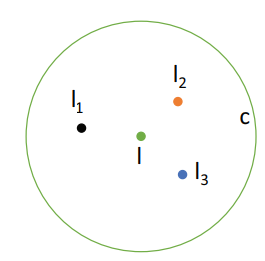
\includegraphics[scale=.6]{figs/figs-2-1.png}
            \label{fig:foo-1}
        }
    \subfloat[Query regions of assisted locations]
        {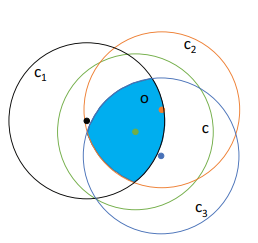
\includegraphics[scale=.6]{figs/figs-2-2.png}
            \label{fig:foo-2}
        }
    \caption{ Assisted locations and their query regions }
    \label{fig:foo}
\end{figure}

Thus, the region $o$ is defined as the accurate region. Moreover, users can set the anticipated query range and the assisted query range according to the different network environment, privacy protection demands and utility demands.  

\textit{\subsection{Adversary model}}
This model assumes that adversaries are strong enough to collect all the information that was sent to LSS providers by users. However, they are not able to collect the parameter settings of users. Thus, adversaries will know the assisted locations $l_1, l_2, l_3$ and the query ranges $(1 + \Delta)r$ of assisted queries. In addition, we assume adversaries also know the principle of this algorithm. Adversaries know the coordinates of three assisted query locations. Then, they can use Trilateration to narrow down the real locations of users according to all the collected data, such that Fig. 2 (b) can be inferred by adversaries. Because three assisted locations are randomly selected in area $c$ and the distances between $l$ and $l_1, l_2, l_3$ are less than $(1 + \Delta)r$, the real location $l$ must be contained within the shadow region
$o$ in Fig. 2 (b).

{\textit{\subsection{Algorithm}}}
According to the proposed algorithm, we will interpret the new definitions and why they are reasonable. In the proposed algorithm, the real location $l$ and the query range $r$ will not be reported to service providers. This algorithm need users get permission to read data from GPS. The raw data from GPS will only be used to generate assisted location. It will not be sent to any service provider.
\\

\textbf{Step 1.} \textit{Before query service, a user initializes its real location $l$ with coordinate $(x_0, y_0)$ and query range $r$.}
\\

\textbf{Step 2.} \textit{Using the real location $l$ and the query range $r$ of the user, randomly selects three assisted locations $l_1, l_2$ and $l_3$. \\
If the three assisted locations $l_1, l_2$ and $l_3$ are in one line, randomly re-select the three assisted locations. \\
The distance between each of these assisted locations and $l$ is less than $r$.} 
\\

\textbf{Step 3.}  \textit{Launch three queries corresponding to the three assisted locations. Each query uses range $(1 + \Delta)r$ instead of the actual query range $r$. The three launched query regions are defined as $c_1, c_2, c_3$.}
\\

\textbf{Step 4.} \textit{The service will receive and respond to the three queries. Thus, the user will receive three query result sets $t_1,t_2,t_3$}. 
\\

\textbf{Step 5.} \textit{Calculate the intersection $t$ of $t_1,t_2,t_3$ where $t = t_1  \cap  t_2 \cap t_3$}
\\
\textbf{Step 6.} \textit{Calculate the coordinates of all locations in set $t$, according to Trilateration.}
\\

Note: In step2, the three assisted locations $l_1,l_2$ and $l_3$ could not fall on one line, as we could not derive unique coordinates for each location in set $t$.
\\
\section{Definitions}
Current works use Euclidean distance between obfuscated locations and real locations to define privacy and utility. They also use Euclidean distance between received locations of service and accurate locations to define quality loss. Actually, when adversaries want to infer the location of users, they usually infer a region rather than a specific location or distance. Therefore, using a region to define privacy is more reasonable than distance. In this paper, all the related definitions are in terms of area. This section will illustrate how to define privacy, utility, quality loss and overhead by using area.

\textit{\subsection{Privacy}}
As shown in Fig. 2(a), a user query service by using location $l$ and query range. Then the algorithm launches three queries by using three assisted-locations $(l_1, l_2, l_3)$ selected in Step 2. The query range is $(1 + \Delta)r$. Therefore, the LSS provider will receive three query regions $(c_1, c_2, c_3)$ as Fig. 2 (b). Then it will send back a set of results for each of the query regions. By using the three service requests, the service provider can derive a prediction of the region of the user. Lemma 1 shows the how the service provider predicts the location region of the user.
\\ \\
\textbf{Lemma 1.} \textit{If a user launches a query by using three assisted regions $(c_1, c_2, c_3)$, let $o = c_1\cap c_2\cap c3$ denote the overlap region of the three assisted query regions. The user must be located in the overlap region $o$.}
\\ \\ 
\textit{Proof.} Users choose three assisted locations $(l_1, l_2, l_3)$ in range
$r$. Thus, the distances between $l$ and $l_1, l_2, l_3$ are less or equal to $r$. Assume S is a set of locations. The distances between each location in $S^\prime$ and $l_1, l_2, l_3$ are less than or equal to $r$. Thus, $l\in S$. Assume $S^\prime$ is also a set of locations. Because the distances between each location in $S^\prime$ and $l_1, l_2, l_3$ are less than or equal to $(1+\Delta)r$, we have $S \in S^\prime$. Therefore, we have $l \in S \in S^\prime$. The set of locations in the overlap region o can be defined by $S^\prime$. Thus, $l$ must be located in region $o$. The lemma is proved. $\qed$
\\ \\

Because adversaries cannot know the parameters of users, they can only use the query range $(1 + \Delta)r$ to infer the real locations of users. According to Lemma 1, users must be located in the overlap region $o = c_1 \cap c_2 \cap c_3.$ Assume each user has a sensitive region $v$. The sensitive region means that if the adversary knows the user is in the sensitive region, the adversary will know the activity of the user. It is obvious to see that:
\[ Pr(\textit{\text{an adversary knows the activity of a user}}) = \frac{v}{o}.\]
As a result, a larger $o$ will decrease the chance of activity prediction of users. Therefore, we can use the area of the region $o$ (as shown in Fig. 3) to define privacy.  \\

\textbf{Definition 1} (Privacy). \textit{Privacy is defined as the area of overlap region of three assisted query regions.
\begin{equation}
    P = Area(o) = Area(c_1 \cap c_2 \cap c_3)
\end{equation}
where $c_1, c_2, c_3$ are assisted query regions and $o = c_1 \cap c_2 \cap c_3$ denotes the overlap region of three assisted query regions.} \\ \\
According to the definition of privacy, a larger region o
means a better privacy protection

\textit{\subsection{Utility}} 

As shown in Fig. 2(b), $c_1, c_2, c_3$ are three assisted query regions of a user. The user will receive a set of results for each of the three regions. According to the Trilateration (refer to Section 3.3), the user can calculate the coordinates of the locations in the overlap region of $c_1, c_2, c_3$. Thus, the user will have accurate services for the overlap region $o = c_1 \cap c_2 \cap c_3$. Even though the information of locations in $o$ is accurate, users do not need the result of locations out of query region as the circle $c$ shown in Fig 4. Only locations in the shadow regions a in Fig. 4 are meaningful to users and have accurate services. Therefore, we can use the area of region a to define the utility (quality of service).
\\

\textbf{Definition 2} (Utility). \textit{Utility is defined as the area of overlap region of the three assisted query region and the anticipative query region.}
\begin{equation}
    U = Area(a) = Area(c \cap c_1 \cap c_2 \cap c_3)
\end{equation}

According to the definition of utility, a larger region a implies a better utility. Furthermore, the utility has a positive correlation with privacy. That means the proposed algorithm does not need to scarify any utility to provide better privacy. Therefore, the proposed algorithm fundamentally solves the trade-off problem between privacy and utility.

\textit{\subsection{Quality Loss}}
In this paper, the proposed algorithm can derive accurate services for the region $a$ as in Fig. 4. However, if $\Delta$ is not larger enough, the accurate region a cannot cover the anticipative query region $c$. Let $q_1 = c -a $. Then the locations in region $q_1$ can be covered by at most two assisted query regions. Because the user can not calculate the coordinates of the locations in region $q_1$, the area $q_1 = c - a$ is defined as an inaccurate region. We use the area of inaccurate region $q_1$ to denote the quality loss of services.
\\

\textbf{Definition 3} (Quality Loss). \textit{Quality loss is defined as the area difference between the anticipative query region and the accurate region.}
\begin{equation}
    QL = Area(q_l) = 
    \left\{
    \begin{array}{ll}
        Area(c-a) & if Area(c-a) > 0
        \\
        0 & if Area(c-a) \le 0,
    \end{array}
    \right.
\end{equation}
\textit{where $c$ denotes the anticipative query region of users and $q_l$ denotes the region which has inaccurate service.}
\\

According to the definition, a larger region a implies less quality loss. The region a is related to the parameter $\Delta$. Users can increase the area of the region $a$ by increasing $\Delta$. If the increased region $a$ is large enough to cover the whole query region c, the quality loss will decrease to zero. However, the increased $\Delta$ will cause high data usage. In the next subsection, we will illustrate how to increase privacy and decrease quality loss by increasing overhead. 

\textit{\subsection{Overhead}}
As Fig. 2(b) shows, $c$ is the anticipative query region of a user. If users do not use the protection algorithm, they only query region $c$ by using the real location $l$ query range $r$. With the proposed protection algorithm, users need to query region $c_1,c_2,c_3$ by using three assisted location $l_1,l_2,l_3$ and query  range $(1+\Delta)r$. Thus, at least three times more area of regions than original query will be queried if users use the proposed protection algorithm. Thus, we need to introduce a new metric to measure the extra query launched by the proposed algorithm.  We define the difference area between actual query region launched by the proposed algorithm and anticipative query region as overhead. 
\\

\textbf{Definition 4} (Overhead). \textit{ Overhead is defined as the area difference between the summation of actual query regions and the anticipative query region.}
\begin{equation}
    O = Area(c_1) + Area(c_2) + Area(c_3) − Area(c).
\end{equation}

\section{Calculation} 
In this section, we will discuss how to calculate the privacy, utility, quality loss and overhead of users. We derive the formulation of expected privacy and quality loss. In addition, we will illustrate how to increase privacy and decrease quality loss by increasing overhead.
The definitions, privacy, utility, quality loss and overhead are related to overlap area of $c_1, c_2$ and $c_3$. Thus, we have to ensure there is an overlap region. \\ \\

\textbf{Lemma 2.} \textit{Assisted query regions $c_1, c_2, c_3$ must have an overlap region.} \\ \\
\textit{Proof.} Assume $S_1$ is the set of locations that distances to $l_1$ are less than $(1 + \Delta)r$; $S_2$ is the set of locations that distances to $l_2$ are less than $(1 + \Delta)r$; $S_3$ is the set of locations that distances to $l_3$ are less than $(1 + \Delta)r$. Then we have $l \in S_1, l \in S_2, l \in S_3.$ Thus, $l \in (S_1 \cap S_2 \cap S_3)$ Obviously, sets of locations in regions $c_1, c_2, c_3$ are the sets $S_1, S_2, S_3$. Because $l \in (S_1 \cap S_2 \cap S_3)$ means $(S_1 \cap S_2 \cap S_3) \neq 0$ , assisted query regions $c_1, c_2, c_3$ must have an overlap region. The lemma is proved. $\qed$


\textit{\subsection{Privacy}} 

Assume the real location $(l(x_0, y_0))$ of a user $l(x_0, y_0)$ is the origin of a Cartesian coordinate system as shown in Fig. 3(a). Assisted locations $l_1(x_1, y_1), l_2(x_2, y_2), l_3(x_3, y_3)$ are randomly selected in the anticipative query region $c$. Mathematically, we can derive the area of region $o$ (the shadow region $o$ in Fig. 3) by using coordinates of assisted locations. Fig. 3 shows the two shapes of overlap region $o$. In Fig. 3(a), the shape of region $o$ is a circular triangle. In Fig. 3(b), the region $o$ is inside of the circle $c_2$. Thus, its shape is a lens. Therefore, we have equation for privacy.
\begin{equation}
P(x_1,y_1,x_2,y_2,x_3,y_3,\Delta, r) =
\left\{
    \begin{array}{l}
        \text{area of circular triangle} & \\
        \text{area of lens,} &
    \end{array}
\right.
\end{equation}
The condition of the two different shape of area can be found in [33]. 
\\
\begin{figure}
\centering
    \subfloat[]
        {
            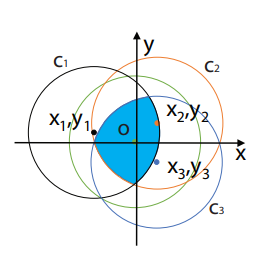
\includegraphics[scale=.6]{figs/figs-3-1.png}
            \label{fig:foo-1}
        }
    \subfloat[]
        {
            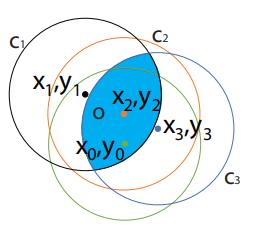
\includegraphics[scale=.6]{figs/figs-3-2.png}
            \label{fig:foo-2}
        }
    \caption{  Two types of overlap region}
    \label{fig:foo}
\end{figure}
\textit{\subsection{Utility}}
According to the definition of utility, we need to calculate the area of overlap region as the shadow regions $o$ shows in Fig.4 $c,c_1,c_2,c_3$. We can see that there are two shapes of overlap region. Fig. 4(a) and Fig. 4(d) have circular quadrangle shapes and Fig. 4(b) and Fig. 4(c) have circular triangle shapes.  Therefore, we have equation for utility.
\begin{equation}
U(x_1,y_1,x_2,y_2,x_3,y_3,\Delta,r) =
\left\{
    \begin{array}{ll}
        \text{area of circular quadrangle} & \\
        \text{area of circular triangle,} &
    \end{array}
\right.
\end{equation}

In the above equation, the overlap area is a circular quadrangle if $c$ has three intersections with $c_1,c_2,c_3$.  
\begin{figure}
\centering
    \subfloat[]
        {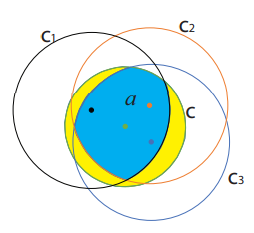
\includegraphics[scale=.6]{figs/figs-4-1.png}
            \label{fig:foo-1}
        }
    \subfloat[]
        {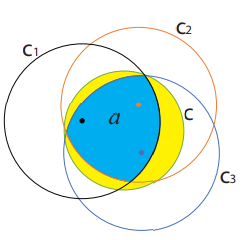
\includegraphics[scale=.6]{figs/figs-4-2.png}
            \label{fig:foo-2}
        }
    \newline
    \subfloat[]
        {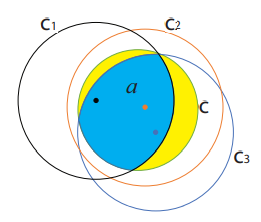
\includegraphics[scale=.6]{figs/figs-4-3.png}
            \label{fig:foo-1}
        }
    \subfloat[]
        {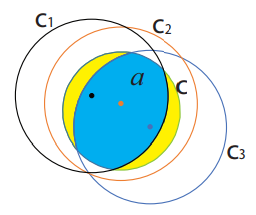
\includegraphics[scale=.6]{figs/figs-4-4.png}
            \label{fig:foo-2}
        }
    \caption{  Four types of Utility}
    \label{fig:foo}
\end{figure}

\textit{\subsection{Quality Loss}}
According to the definition of quality loss, the region that belongs to anticipative query region  but not covered by accurate region is defined as quality loss. We can derive the equation of quality loss. 
\begin{equation}
    QL(x_1,y_1,x_2,y_2,x_3,y_3,\Delta,r) = 
    \left\{
    \begin{array}{ll}
        \pi R^2-U & if \pi R^2 > U \\
        0 & if \pi R^2 \le U,
    \end{array}
    \right.
\end{equation}
where $R = (1+\Delta)r$ is the assisted query range and $U$ is the function of accurate area $U(x_1,y_1,x_2,y_2,x_3,y_3,\Delta,r)$. 

\textit{\subsection{Overhead}}
In this paper, we use the area of excess query region to measure the excess data usage of users. Therefore,we have the equation for overhead.  
\begin{equation}
    O(\Delta, r) = 3\pi (1+\Delta)^2r^2 - \pi r^2. 
\end{equation} \\

$\Delta$ can be used to balance the trade-offs between privacy and overhead and quality loss and overhead. User can increase privacy and utility and decrease quality  loss by increasing overhead. We will discuss the tradeoffs in the next subsection. 

\textit{\subsection{Expectation of Privacy and Utility}}
Because the algorithm randomly selects assisted locations
from the circle region with center $l$ and range $r$, the probability of choosing assisted locations is uniform distributed. The area of the circle region with center $l$ and range $r$ is $\pi r^2$. Therefore, the probability density of randomly choosing any three assisted locations is $(\frac{1}{\pi r^2})^3$. Then we derive the equation for the expected privacy and expected utility. 
\begin{equation}
    P_{exp}=\iint_{x_{3}^{2}+y_{3}^{2} \leqslant r^{2}} \iint_{x_{2}^{2}+y_{2}^{2} \leqslant r^{2}}  \iint_{x_{1}^{2}+y_{1}^{2} \leqslant r^{2}}\left(\frac{1}{\pi r^{2}}\right)^{3} P(\ldots) D,
\end{equation}
\begin{equation}
    U_{exp} = \iint_{x_{3}^2 + y_{3}^2\leqslant r^2}\iint_{x_{2}^2+y_{2}^{2}\leqslant r^2} \iint_{x_{1}^{2} + y_{1}^{2} \leqslant r^2} \left(\frac{1}{\pi r^2} \right) ^3 U(\ldots)D,
\end{equation}
where $D = d_{x_1} d_{y_1}d_{x_2}d_{y_2}d_{x_3}d_{y_3},$ \\ 
$P(\ldots)$ denotes $P(x_1,y_1,x_2,y_2,x_3,y_3,\Delta,r)$ and \\
$U(\ldots)$ denotes $U(x_1,y_1,x_2,y_2,x_3,y_3,\Delta,r)$.

\textit{\subsection{Area Calculation}}
Two kinds of shapes need to be calculated for privacy: lens (shadow region $o$ in Fig. 3 (b)) and circular triangle (shadow region $o$ in Fig. 3 (a)). If $\Delta<1$, two kinds of shapes also need to be calculated for utility: circular triangle (shadow region $o$ in Fig. 4 (b) (c)) and circular quadrangle (shadow region $o$ in Fig. (a) (d)). If $\Delta>1$, we only just need to calculate the anticipative query region (the circle $c$ region in Fig. 5 (b)) for utility because the assistant query regions cover all the anticipative query regions. \\ \\
\textit{\subsubsection{Area of lens}}
For the area of lens, we can calculate using following steps: \\ \\
\textbf{Step 1.} \textit{Calculate the two intersection points.} \\ \\
\textbf{Step 2.} \textit{Calculate the distance $d$ between two intersection points. } \\ \\
\textbf{Step 3.} \textit{Calculate the area of circular segment:}
\begin{equation}
    A_{seg} = r^2 cos^{-1} \frac{\sqrt{4r^2 - d^2}}{2r} - \frac{d\sqrt{4r^2-d^2}}{4}.
\end{equation}
Because the lens is informed by two circles having the same radius, the area of lens is 
\begin{equation}
    A_{lens} = 2A_{seg}.
\end{equation}
\textit{\subsubsection{Area of circular triangle}}
Fewell derived the closed-form algebraic expression of the
area of common overlap of three circles [33]. Assume
$d_12, d_23, d_13$ are the distances between the center points of circle 1 and circle 2, circle 2 and circle 3 and circle 1 and circle 3. \\ \\ 
\textbf{Step 1.} \textit{Calculate the intersection point of circles 1 and 2}
\[
\left\{
    \begin{array}{ll}
        x_{12} = \frac{r_1^2 - r_2^2 + d_{12}^2} {2d_{12}} & \\
        y_{12} = \frac{1}{2d_{12}} \sqrt{2d_{12}^2 (r_1^2 + r_2^2)-(r_1^2 - r_2^2)-d_{12}^4} & 
    \end{array}
\right.
\]
\textbf{Step 2.} \textit{Calculate the sines and cosines of the angles $\theta^{\prime}$ (between $d_{12}$ and $d_{13}$) and $\theta^{\prime \prime}$ (supplementary angle of angle between $d_{23}$ and $d_{13}$)}
\[
\left\{
    \begin{array}{l}
         cos\theta^\prime = \frac{d_{12}^2 + d_{13}^2 - d_{23}^2}{2d_{12}d_{12}} \\ \\
         cos\theta^{\prime\prime} = - \frac{d_{12}^2 + d_{23}^2 - d_{13}^2}{2d_{12}d_{23}} \\ \\
         sin\theta^\prime = \sqrt{1-cos^2\theta^\prime} \\ \\
         sin\theta^\prime = \sqrt{1-cos^2\theta^{\prime\prime}}.
    \end{array}
\right.
\] \\ \\
\textbf{Step 3} \textit{Calculate the coordinate of the intersection points involving circle 3}
\[
\left\{
\begin{array}{l}
    x_{13}^{\prime}=\frac{r_{1}^{2}-r_{3}{ }^{2}+d_{13}{ }^{2}}{2 d_{13}} \\
    y_{13}^{\prime}=\frac{-1}{2 d_{13}} \sqrt{2 d_{13}^{2}\left(r_{1}^{2}+r_{3}^{2}\right)-\left(r_{1}^{2}-r_{3}^{2}\right)^{2}-d_{13}^{2}} \\
    x_{13}=x_{13}^{\prime} \cos \theta^{\prime}-y_{13}^{\prime} \sin \theta^{\prime} \\
    y_{13}=x_{13}^{\prime} \sin \theta^{\prime}+y_{13}^{\prime} \cos \theta^{\prime} \\
    x_{23}^{\prime \prime}=\frac{r_{2}{ }^{2}-r_{3}{ }^{2}+d_{23}{ }^{2}}{2 d_{23}} \\
    y_{23}^{\prime \prime}=\frac{-1}{2 d_{23}} \sqrt{2 d_{23}^{2}\left(r_{2}^{2}+r_{3}^{2}\right)-\left(r_{2}^{2}-r_{3}^{2}\right)^{2}-d_{23}^{2}} \\
    x_{23}=x_{23}^{\prime \prime} \cos \theta^{\prime}-y_{23}^{\prime \prime} \sin \theta^{\prime} \\
    y_{23}=x_{23}^{\prime \prime} \sin \theta^{\prime}+y_{23}^{\prime \prime} \cos \theta^{\prime} .
\end{array}
\right.
\] \\ \\
\textbf{Step 4.} \textit{Use the coordinates of the intersection points to calculate the chord length $c_1,c_2,c_3$}
\[
c_k^2 = (x_{ik} - x_{jk})^2 + (y_{ik}-y_{jk})^2.
\] \\ \\
\textbf{Step 5.} \textit{Determine whether} 
\begin{equation}
    d_{13}sin\theta^\prime < y_{13} + \frac{y_{23}-y_{13}}{x_{23}-x_{13}} (d_{13}cos\theta^\prime - x_{13})
\end{equation}
\textit{is true or false.} \\ \\

\textbf{Step 6.} \textit{The area of circular triangle $A_{Ctri}$ is given by}

\[
\begin{aligned}
    &\frac{1}{4} \sqrt{(c_{1}+c_{2}+c_{3})(c_{2}+c_{3}-c_{1})(c_{1}+c_{3}-c_{2})(c_{1}+c_{2}-c_{3})} \\
    &\left.+\prod_{k=1}^{3}\left(r_{k}^{2} \arcsin \frac{c_{k}}{2 r_{k}}\right)-\prod_{k=1}^{2} \frac{c_{k}}{4} \sqrt{4 r_{k}^{2}-c_{k}^{2}}\right) \\
    & +
\left\{
    \begin{aligned}
         \frac{c_{3}}{4} \sqrt{4 r_{3}^{2}-c_{3}^{2}} &(\textit { Eq.8 is true }) \\
         \frac{-c_{3}}{4} \sqrt{4 r_{3}^{2}-c_{3}^{2}} &(\textit { Eq.8 is false })
    \end{aligned}
\right.
\end{aligned}
\] \\ \\
\textbf{\subsubsection{Area of circular quadrangle}}
A circular quadrangle is composed by one quadrangle and four segments. The area of circular quadrangle can be derived by the following steps: \\ \\
\textbf{Step 1.} \textit{Calculate the four intersection points Step 2. Calculate the area of quadrangle which uses $\left(x_{0}, y_{0}\right),\left(x_{1}, y_{1}\right), \\ \left(x_{2}, y_{2},\left(x_{3}, y_{3}\right)\right.$ as vertexes of the four circle.} \\ \\
\begin{figure}
\centering
    \subfloat[Assisted locations]
        {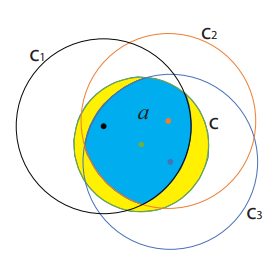
\includegraphics[scale=.6]{figs/figs-5-1.png}
            \label{fig:foo-1}
        }
    \subfloat[Query regions of assisted locations]
        {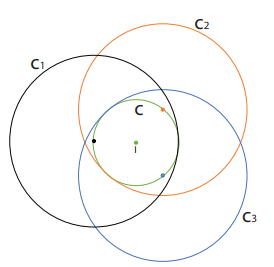
\includegraphics[scale=.6]{figs/figs-5-2.png}
            \label{fig:foo-2}
        }
    \caption{ Privacy difference and quality loss difference between different query ranges}
    \label{fig:foo}
\end{figure}

\textbf{Step 2.} \textit{Calculate the area of quadrangle which uses $(x_0,y_0),(x_1,y_1),(x_2,y_2),(x_3,y_3)$ as vertexes.} \\
$
A_{q a}= \\ \frac{1}{2}\left(\left|
\begin{array}{ll}
x_{0} & x_{1} \\
y_{0} & y_{1}
\end{array}\right
|+\left|\begin{array}{ll}
x_{1} & x_{2} \\
y_{1} & y_{2}
\end{array}\right|+\left|\begin{array}{ll}
x_{2} & x_{3} \\
y_{2} & y_{3}
\end{array}\right|+  \left|\begin{array}{ll}
x_{3} & x_{1} \\
y_{3} & y_{1}
\end{array}\right|\right) .
$
\textbf{Step 3.} \textit{Calculate the distance $d_{i}$ between any two adjacent intersection points; $d_{i}$ means the according arc string belongs to circle $i, i \in 0,1,2,3$.} \\ \\
\textbf{Step 4.} \textit{Use Equation (7) to calculate the area of four segments:}
$$
A_{segs}=\prod_{i=0}^{3} A_{s e g}\left(r_{i}, d_{i}\right) .
$$
Therefore, the area of circular quadrangle is:
$$
A_{\text {Cirq }}=A_{q a}+A_{\text {segs } } .
$$
For the program of all the calculations, please see [34].

\section{Tradeoffs and discussion}
As the proposed algorithm fundamentally solved the tradeoff problem between privacy and utility, we now consider the
tradeoff between privacy and overhead and the tradeoff between
quality loss and overhead.
\textit{\subsection{Tradeoff between Privacy and Overhead}}
Users choose assisted locations in range $r$ and query services with range $(1+\Delta) r$. If $\Delta=0$, users have the assisted query regions as shown in Fig. 2(b). If $\Delta>0$, users have the assisted query regions as shown in Fig. 5(a). Obviously, the overlap region $o$ in Fig. 5(a) is larger than the overlap region $o$ in Fig. 2(b). Actually, users can obtain a larger expected privacy if they use a larger $\Delta$.
\\ \\ 
\textbf{Theorem 1.} \textit{If $\Delta^{\prime \prime} > \Delta^\prime, \text{then} P_{exp}(\ldots,\Delta^{\prime \prime},r) < P_{exp}(\ldots,\Delta^{\prime},r).$} \\ \\ 
\textit{Proof.} Let $P^\prime = P(x_1,y_1,x_2,y_2,x_3,y_3,\Delta^\prime,r)$ and $P^{\prime \prime} = P(x_1,y_1,x_2,y_2,x_3,y_3,\Delta^{\prime \prime},r)$ Because $\frac{1}{\pi r^2} P(\ldots) > 0)$, we can prove 
\[
\iint \iint \iint (\frac{1}{\pi r^2})^3 p^{\prime \prime}D > \iint \iint \iint (\frac{1}{\pi r^2})^3 p^{\prime}D,
\]
where $D=d_{x_{1}} d_{y_{1}} d_{x_{2}} d_{y_{2}} d_{x_{3}} d_{y_{3}}$. $\qed$ \\ \\

According to Theorem 1, users can increase the parameter $\Delta$ to increase the protection strength.
\textit{\subsection{Tradeoff between Quality Loss and Overhead}}
Users can also use $\Delta$ to balance the tradeoff between utility and overhead. As shown in Fig. 5, Fig. 5(b) has less QL than Fig. 5(a) because Fig. 5(b) has larger $\Delta$ than Fig. 5(a). \\ \\
\textbf{Theorem 2.} \textit{If $\Delta^{\prime \prime}>\Delta^{\prime}$, then $U_{\exp }\left(\ldots, \Delta^{\prime \prime}, r\right)>U_{\exp }\left(\ldots, \Delta^{\prime}, r\right)$.} \\ \\

According to the equation of quality loss, we can derive the following theorem:

\textbf{Theorem 3.} If $\Delta^{\prime \prime}>\Delta^{\prime}$ and $Q L_{e x p}\left(\ldots, \Delta^{\prime}, r\right) \neq 0$, then $Q L_{\exp }\left(\ldots, \Delta^{\prime \prime}, r\right)<Q L_{\exp }\left(\ldots, \Delta^{\prime}, r\right)$.

We can prove Theorem 2 and Theorem 3 as the proof of Theorem 1 . According to Theorem 3 , users can increase $\Delta$ to obtain less QL. Furthermore, the quality loss will decrease as the value of $\Delta$ increases until quality loss is equal to 0 . \\ \\ 
\textbf{Theorem 4.} If $\Delta=1$, then $Q L=0$. \\

Proof. As Fig. 5(b) shows, if users use $2 r$ as the assisted query range, $c \in c_{1}, c \in c_{2}, c \in c_{3}$. Then we have $c \in c_{1} \cap c_{2} \cap c_{3}$. That means the overlap region $o$ of assisted query regions will cover the whole anticipative query region $c$. Thus, the quality loss $Q L=0$. $\qed$ \\ \\

When $\Delta=1$, the overhead is $11 \pi r^{2}$. That means users can obtain the accurate LSSs with zero quality loss in an Internet environment that can tolerate $11 \pi r^{2}$ overhead. Due to the large coverage of Wi-Fi and inexpensive data of the fourth generation of mobile telecommunications technology (4G), the condition of the Internet environment is easy to be satisfied.
\\
\section{Simulation}

Most of the current algorithms need to be deployed in the Operating System (OS) level of mobile phones. However, there is no secure way to make a system level change in either Android devices or iOS devices. In the Android OS, users need to open the root authority to make system level change, thereby introducing many more privacy issues. Any application can get the private information and raw data from sensor easily in an open root authority Android device. In the iOS, users cannot make any system level change. The only way to install a system level application is hacking the system. However, a hacked iOS has no protection. We could not install a privacy protection algorithm by making the system vulnerable.

The algorithm proposed in this paper can be deployed in the application without system level change if the application has permission to read GPS
\begin{figure}
    \centering
    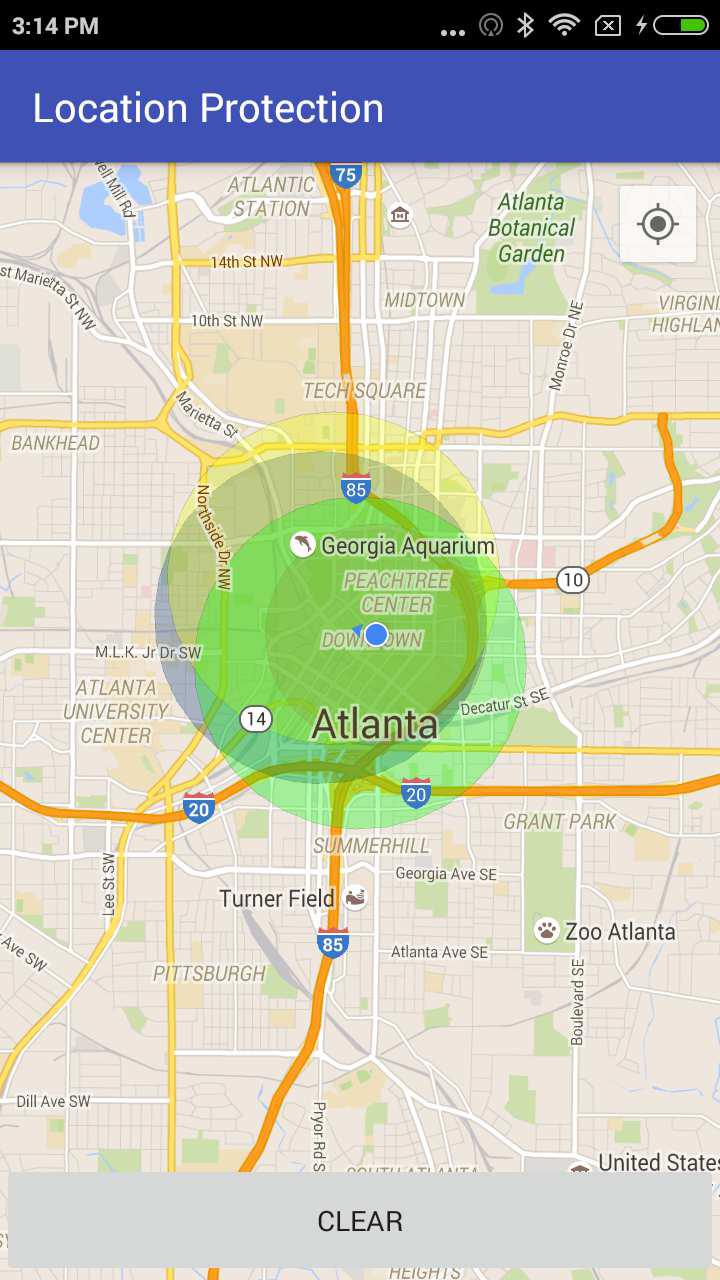
\includegraphics[scale=.9]{figs/figs-6-1.png}
    \caption{Demo of privacy protection in Android.}
    \label{fig:my_label}
\end{figure}
information. The location data from GPS will be kept in local and will not be sent to the service provider. Based on the Google Map service, we built a demo to install our proposed algorithm in an Android device as shown in Fig. 6. To illustrate how the proposed algorithm works, we draw circles above the map layer. The blue dot is the real location of the current user. The real location is determined from GPS of the device. The small circle covered by three big circles is the anticipative query region launched by using the real location and query range $r$. The three big circles are assisted query region launched by using three assisted locations and query range $(1+\Delta) r$ where $\Delta=0.5$. Users can set the value of $\Delta$ according to different privacy and service quality demands we discussed in Section 6. The demo is in [34].
\begin{figure}
\centering
    \subfloat[Expected Privacy]
        {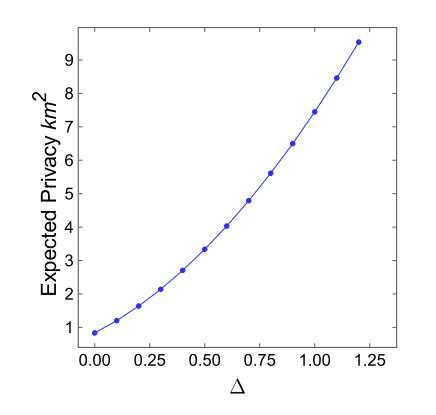
\includegraphics[scale=.4]{figs/figs-7-1.png}
            \label{fig:foo-1}
        }
    \subfloat[Expected Quality Loss]
        {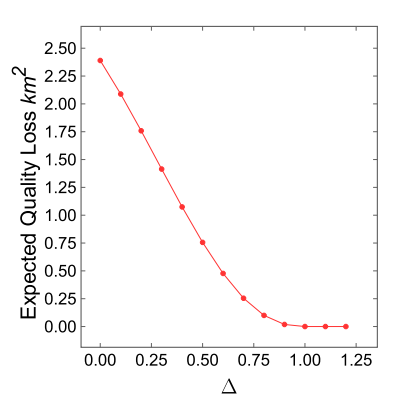
\includegraphics[scale=.4]{figs/figs-7-2.png}
            \label{fig:foo-2}
        }
    \caption{ Expected Privacy and Quality Loss as $\Delta$ increases when r = 1km }
    \label{fig:foo}
\end{figure}

Due to the complexity of expectation calculations of privacy and QL, we wrote a program to calculate the expectation of privacy and $\mathrm{QL}$ and used the program to calculate privacy and QL 50 million times. We then derived the expected privacy and QL by calculating the average value of the 50 million results.

Fig. 7 shows the results for expected privacy and $\mathrm{QL}$ as $\Delta$ increases when query range $r=1 \mathrm{~km}$. As shown in Fig. 7 (a), as $\Delta$ increases, expected privacy increases exponentially. Fig. 7 (b) shows that QL decreases exponentially as $\Delta$ increases and $\mathrm{QL}$ decreases to 0 when $\Delta$ is greater than 1 because all the three assisted query regions can cover the original query region. The decreased QL also means the utility is increased with $\Delta$ increasing. We can know from Fig. 7, a larger $\Delta$ can provide better privacy protection with less QL. Besides, the QL can be 0 if the value of $\Delta$ is large enough.

The results also illustrate that adversaries can hardly infer the location of users. As shown in Fig. 7(a), the privacy is larger than $4 \mathrm{~km}^{2}$ when $\Delta$ is larger than $0.6$. If we assume that the sensitive region $v$ of users is a $4000 \mathrm{~m}^{2}$ region around users, the probability that adversaries can infer the right region of users is less than $0.001$. The $\mathrm{QL}$ is less than $0.5 \mathrm{~km}^{2}$ when $\Delta$ is larger than 0.6. Because the area of original query region is larger than $\pi r^{2}=3.14 \mathrm{~km}^{2}$. Therefore, the quality loss is less than $16 \%$ of original query region. Users still can decrease the quality loss by increasing $\Delta$.
\begin{figure}
\centering
    \subfloat[Expected Privacy]
        {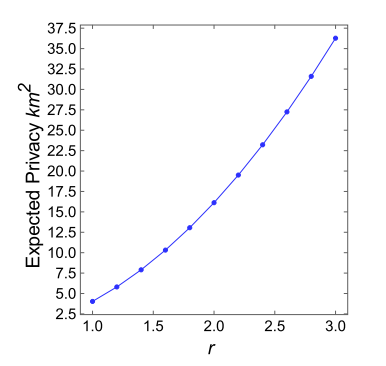
\includegraphics[scale=.4]{figs/figs-8-1.png}
            \label{fig:foo-1}
        }
    \subfloat[Expected Quality Loss]
        {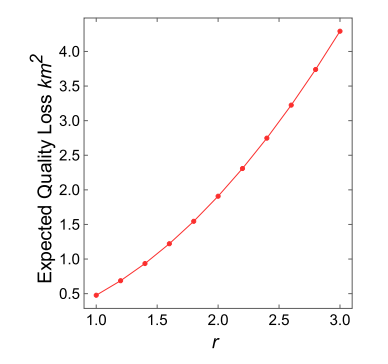
\includegraphics[scale=.4]{figs/figs-8-2.png}
            \label{fig:foo-2}
        }
    \caption{ Expected Privacy and Quality Loss as $r$ increases when $\Delta = 0.6$.}
    \label{fig:foo}
\end{figure}

\begin{figure}
\centering
    \subfloat[Overhead as $\Delta$ increases]
        {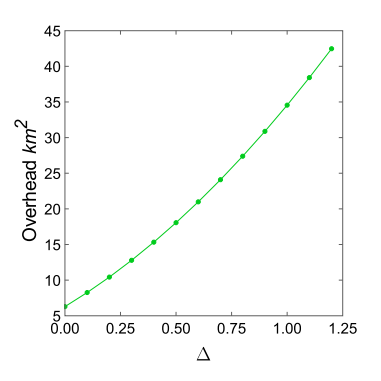
\includegraphics[scale=.4]{figs/figs-9-1.png}
            \label{fig:foo-1}
        }
    \subfloat[Overhead as$r$ increases]
        {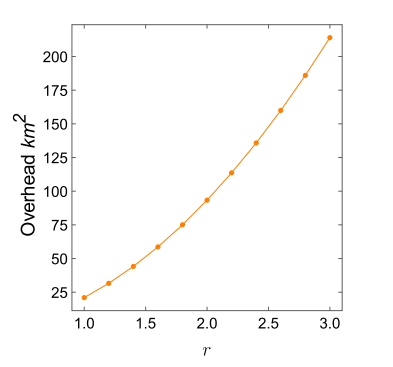
\includegraphics[scale=.4]{figs/figs-9-2.png}
            \label{fig:foo-2}
        }
    \caption{Overhead as $\Delta$ and $r$ increase }
    \label{fig:foo}
\end{figure}

Fig. 8 shows the results of expected privacy and expected $\mathrm{QL}$ as $r$ increases when $\Delta=0.6$. As shown in Fig. 8 (a), expected privacy increases exponentially as $r$ increases. This means a larger $r$ can also lead to a better privacy protection. However, expected $\mathrm{QL}$ will increases exponentially as $r$ increases as shown in Fig. 8 (b). This is because the increased query range $r$ will decrease the intersection region between anticipated query region and assisted query region due to a fixed $\Delta$. As a result, users can still get strong privacy protection when they use a large $r$, causing the utility to decrease accordingly. Thus, if users want to increase privacy protection, they should increase the value of $\Delta$ instead of $r$. Besides, when users launch a query for a large region, they need also increase the value of $\Delta$ to offset the increased quality loss caused by a large query range.

As we discussed in Section IV, larger $\Delta$ and $r$ will lead to larger overhead. Fig. 9 plots the overhead as $\Delta$ and $r$ increase. We can see from Fig. 9, overhead also increases exponentially as $r$ and $\Delta$ increase. Therefore, if users have limited data usage and bandwidth, they should consider the large overhead caused by a large value of $\Delta$. Especially when users want to increase privacy protection by increasing the query range $r$, they should use a large $\Delta$ to offset the QL. If users can tolerate the Overhead, they can use a large value for both the query range $r$ and $\Delta$ to increase their privacy protection.

\section *{Acknowledgments}
This work is partly supported by the National Science Foundation (NSF) under grant NOs 1252292, 1741277 and 1704287. 

\nocite{bugliesi2006automata,zhang2016fakemask,gedik2007protecting,vu2012efficient,he2016cost,soria2014enhancing,he2017latent,jorgensen2015conservative,liang2017location,junglas2008location,zheng2017follow,danezis2012financial,lamarca2007pervasive,feng2016relationship,yin2017location, zhang2010location,zheng2019privacy,niu2014achieving,chen2013privacy,ma2010privacy,trujillo2013privacy,yuan2011protecting,chatzikokolakis2013broadening,li2014data,dewri2012local,andres2013geo,fawaz2014location,li2013search,ardagna2007location,ardagna2008privacy,ardagna2009obfuscation,fang1986trilateration,fewell2006area}

%% Loading bibliography style file
%\bibliographystyle{model1-num-names}
\bibliographystyle{cas-model2-names}

% Loading bibliography database
\bibliography{Reference.bib}

\end{document}

